\documentclass[12pt,a4paper]{article}
\usepackage[a4paper,total={160mm,250mm}]{geometry}
\usepackage[utf8]{inputenc}
\usepackage[ruled,vlined]{algorithm2e}
\usepackage{amsmath}
\usepackage{amsthm}
\usepackage{amsfonts}
\usepackage{amssymb}
\usepackage{amscd}
\usepackage{color}
\usepackage{enumerate}
\usepackage{graphicx}
\usepackage{hyperref}
\usepackage{listings}
\usepackage{mathtools}
\usepackage{ngerman}

\theoremstyle{definition}
\newtheorem{aufgabe}{Aufgabe}

\theoremstyle{definition}
\newtheorem*{losung*}{Lösung}

\definecolor{mygreen}{rgb}{0,0.6,0}
\definecolor{mygray}{rgb}{0.5,0.5,0.5}
\definecolor{mymauve}{rgb}{0.58,0,0.82}
\definecolor{lightgray}{rgb}{0.9,0.9,0.9}

\lstdefinestyle{python}{
	backgroundcolor=\color{lightgray},   % choose the background color; you must add \usepackage{color} or \usepackage{xcolor}; should come as last argument
	basicstyle=\footnotesize\ttfamily,        % the size of the fonts that are used for the code
	breakatwhitespace=false,         % sets if automatic breaks should only happen at whitespace
	breaklines=true,                 % sets automatic line breaking
	captionpos=b,                    % sets the caption-position to bottom
	commentstyle=\color{mygreen},    % comment style
	deletekeywords={...},            % if you want to delete keywords from the given language
	escapeinside={\%*}{*)},          % if you want to add LaTeX within your code
	extendedchars=true,              % lets you use non-ASCII characters; for 8-bits encodings only, does not work with UTF-8
	firstnumber=1,                   % start line enumeration with line 1000
	frame=single,	                 % adds a frame around the code
	keepspaces=true,                 % keeps spaces in text, useful for keeping indentation of code (possibly needs columns=flexible)
	keywordstyle=\color{blue},       % keyword style
	language=Python,                 % the language of the code
	morekeywords={*,...},            % if you want to add more keywords to the set
	numbers=left,                    % where to put the line-numbers; possible values are (none, left, right)
	numbersep=5pt,                   % how far the line-numbers are from the code
	numberstyle=\tiny\color{mygray}, % the style that is used for the line-numbers
	rulecolor=\color{black},         % if not set, the frame-color may be changed on line-breaks within not-black text (e.g. comments (green here))
	showspaces=false,                % show spaces everywhere adding particular underscores; it overrides 'showstringspaces'
	showstringspaces=false,          % underline spaces within strings only
	showtabs=false,                  % show tabs within strings adding particular underscores
	stepnumber=1,                    % the step between two line-numbers. If it's 1, each line will be numbered
	stringstyle=\color{mymauve},     % string literal style
	tabsize=4,	                     % sets default tabsize to 2 spaces
	title=\lstname,                   % show the filename of files included with \lstinputlisting; also try caption instead of title
	rangeprefix=\#---,
	rangesuffix=---,
	includerangemarker=false
}

\pagestyle{empty}

\title{Raytracing und Vektorgeometrie}
\author{Oliver Rietmann}
\date{\today}

\begin{document}
\maketitle
\tableofcontents

\section*{Einleitung}
Dieses Skript richtet sich an gymnasiale Mittelschüler die mit den grundlegenden Begriffen Vektorgeometrie im dreidimensionalen euklidischen Raum vertraut sind.
Ziel ist es, die Vektorgeometrie zu veranschaulichen indem wir eine konkrete Anwendung in der Computergrafik betrachten, das Raytracing.
Dabei handelt es sich um eine Technik zur Generierung von realistischen 3D Bildern, welche im nächsten Kapitel genauer erklärt wird.
Wir werden den Raytracing-Algorithmus selber implementieren und damit solche Bilder generieren.
Wir verwenden dazu die Programmiersprache Python, welche in Kapitel~\ref{sec:einfuerung} kurz eingeführt wird.
Grundkenntnisse im Programmieren werden dabei vorausgesetzt.
Wer noch nie programmiert hat, kann das zum Beispiel mit der vielen online-Tutorials nachholen, bestenfalls gleich in Python.

\section{Raytracing}
Raytracing bezeichnet eine Methode zur Generierung von realistischen 3D Bildern.
Dabei kommen unter anderem Reflexions- und Brechungsgesetze aus der Physik zur Anwendung.
Vor allem aber beruht die Technik auf der Vektorgeometrie wie man sie am Gymnasium unterrichtet.
Die Idee ist folgende: Wir verteilen einige Objekte (Kugeln, Würfel, etc.) im dreidimensionalen Raum.
Wir nennen dies die Szene.
Nun stellt man irgendwo eine Kamera auf.
Vor der Kamera stellen wir uns eine rechteckige Fläche, die Bildebene, vor.
Auf die Bildebene zeichnen wir nun die dahinter liegende Szene wie folgt:
Ausgehend von der Kamera senden wir einen Strahl aus, der die Bildebene durchstösst und dann womöglich auf ein Objekt unserer Szene trifft.
Trifft der Strahl zum Beispiel auf ein rotes Dreieck, so wird der Durchstosspunkt auf der Bildebene rot eingefärbt.
Danach senden wir einen weiteren Strahl von der Kamera durch einen anderen Punkt auf der Bildebene und färben den Durchstosspunkt entsprechend ein.
Wir wiederholen dies bis die ganze Bildebene eingefärbt ist.
Das so auf der Bildebene generierte Abbild der Szene ist der Output unseres Programms.
Diese Methode ein Bild zu generieren heisst Raytracing, denn man verfolgt den Strahl.
\begin{figure}[h!]
	\centering
	\includegraphics[width=\textwidth]{images/raytracing.png}
	\caption{Raytracing: Es werden Strahlen ausgesendet und deren Schnittpunkte mit Objekten ermittelt. In diesem Fall wir der Durchstosspunkt auf der Bildebene in der Farbe des roten Dreiecks gefärbt.}
	\label{fig:raytracing}
\end{figure}

\section{Eine Einführung in Python 3}\label{sec:einfuerung}
Nun installieren wir Python (Version 3.8 oder höher) und die von unserem Raytracing-Programm benötigten Packages \texttt{numpy} und \texttt{PIL}.
Je nach Betriebssystem muss dabei anders vorgegangen werden.

\subsubsection*{Windows 10}
Gehen Sie auf die offizielle Python-Webseite um von dort die neuste Python Version zu installieren.
Danach überprüfen wir mit folgenden drei Schritten, ob die Installation erfolgreich war:
\begin{enumerate}
	\item Drücken Sie die Windows-Taste um eine Suche zu starten.
	\item Schreiben Sie dann \texttt{cmd} und drücken Sie Enter um die Kommandozeile zu öffnen.
	\item In der Kommandozeile schreiben Sie \texttt{python} und drücken wieder Enter.
\end{enumerate}
Nun sollte die Version der Python-Installation ausgegeben werden.
Anschliessend können in der Kommandozeile mit
\begin{verbatim}
	python -m pip install numpy Pillow --user
\end{verbatim}
die Abhängigkeiten installiert werden.
Von nun an kann ein Python-Script \texttt{script.py} in der Kommandozeile ausgeführt werden mit dem Befehl \texttt{python script.py}.
Dazu muss aber zuerst mit dem Befehl \texttt{cd <Verzeichnis>} in das Verzeichnis navigiert werden, welches \texttt{script.py} enthält.

\subsubsection*{MacOS}
Öffnen Sie einen Terminal, zum Beispliel indem Sie nach der Applikation Terminal suchen.
Installieren Sie dann Homebrew indem Sie die Zeile (alles soll auf eine Zeile!)
\begin{verbatim}
	/bin/bash -c "$(curl -fsSL https://raw.githubusercontent.com/Homebrew/
install/master/install.sh)"
\end{verbatim}
im den Terminal kopieren und mit Enter ausführen.
Anschliessend können Sie Python mit dem Befehl \texttt{brew install python} installieren.
Danach müssen noch mit
\begin{verbatim}
	python3 -m pip install numpy Pillow --user
\end{verbatim}
die Abhängigkeiten installiert werden.
Von nun an kann ein Python-Script \texttt{script.py} im Terminal ausgeführt werden mit dem Befehl \texttt{python3 script.py}.
Dazu muss aber zuerst mit dem Befehl \texttt{cd <Verzeichnis>} in das Verzeichnis navigiert werden, welches \texttt{script.py} enthält.

\subsubsection*{Linux}
Öffnen Sie einen Terminal.
Unter Ubuntu wird Python mit dem Befehl \texttt{sudo apt-get install python3} installiert, unter Fedora hingegen mit \texttt{sudo dnf install python3}.
In beiden Fällen werden Administrator-Rechte benötigt.
Anschliessend können mit
\begin{verbatim}
	python3 -m pip install numpy Pillow --user
\end{verbatim}
die Abhängigkeiten installiert werden.
Von nun an kann ein Python-Script \texttt{script.py} im Terminal ausgeführt werden mit dem Befehl \texttt{python3 script.py}.
Dazu muss aber zuerst mit dem Befehl \texttt{cd <Verzeichnis>} in das Verzeichnis navigiert werden, welches \texttt{script.py} enthält.

\subsection{Listen und Schleifen}
Öffnen Sie nun einen beliebigen Texteditor und erstellen Sie ein File namens \texttt{script.py} das nur folgende Zeile enthält:
\begin{lstlisting}[style=python]
print("Hello World")
\end{lstlisting}
Wenn Sie dieses im Terminal ausführen wie oben beschrieben, sollte die Nachricht \texttt{Hello World} erscheinen.
Die Endung \texttt{.py} kennzeichnet das File als Python-Skript.
Mit der Funktion \texttt{print} kann Text, eine Zahl, und vieles mehr im Terminal ausgegeben werden.
Zum Beispiel können wir eine Liste von Zahlen ausgeben:
\begin{lstlisting}[style=python]
l = [4, 2, 5, 9, 6, 2]
print(l)
\end{lstlisting}
Mithilfe der Klammern \texttt{[ ]} haben wir hier die Variable \texttt{l} definiert und schliesslich mit \texttt{print} ausgegeben.
Mit den Klammern \texttt{[ ]} kann man zudem auf die einzelnen Elemente der Liste zugreifen:
\begin{lstlisting}[style=python]
l = [4, 2, 5, 9, 6, 2]
print(l[0])
print(l[1])
print(l[2])
\end{lstlisting}
Die \texttt{for} Schleife erlaubt es eine Liste zu durchlaufen:
\begin{lstlisting}[style=python]
l = [4, 2, 5, 9, 6, 2]
for i in l:
	print(i)
\end{lstlisting}
Die Variable \texttt{i} durchläuft alle Werte der Liste \texttt{l}.
Man beachte, dass die letzte Zeile eingerückt ist.
Um aus einer Liste von Zahlen einen Vektor zu machen mit dem man rechnen kann, verwenden wir das Package numpy:
\begin{lstlisting}[style=python]
from numpy import array
l = [4, 2, 5, 9, 6, 2]
v = array(l)
print(2 * v)
\end{lstlisting}
So wird das \texttt{numpy.array}, bzw. der Vektor \texttt{v} mit dem Skalar \texttt{2} multipliziert.
Man beachte, das die gewöhnliche Liste \texttt{l} diese Operation nicht unterstützt (probieren Sie!).
Numpy stellt viele weitere Operationen aus der Vektorgeometrie zur Verfügung.
Wie man auf diese zugreifen kann, schaut man am besten im Internet nach.
In jedem Fall müssen diese aber zuerst importiert werden, so wie wir \texttt{numpy.array} in in der ersten Zeile importieren mussten.
Nun folgen noch ein paar wichtige Beispiele:
\begin{lstlisting}[style=python]
from numpy import array, inner
from numpy.linalg import norm
v = array([1, 2, 3])
w = array([4, 5, 6])
print(w - 2 * v)
print(inner(v, w)) # Skalarprodukt von v und w
print(norm(v))     # Betrag des Vektors v
\end{lstlisting}
Der Hashtag \texttt{\#} markiert einen Kommentar, das heisst alle darauffolgenden Zeichen werden ignoriert.

\subsection{Funktionen und Klassen}
Funktionen sind ein Weg um Code-Repetition zu verhindern.
So könnte es zum Beispiel sehr oft nötig sein, einen Vektor zu normieren (das heisst auf Länge 1 zu bringen).
In diesem Fall lohnt es sich, dafür eine Funktion zu machen:
\begin{lstlisting}[style=python]
from numpy import array
from numpy.linalg import norm

def normalize(v):
	return v / norm(v)

w = array([1, 2, 3])
n = normalize(v)
print(n)
\end{lstlisting}
Wir haben also eine Funktion \texttt{normalize} definiert, welche einen beliebigen Vektor (ausser den Nullvektor) auf Länge 1 bringt.
Wie schon beim der \texttt{for} Schleife ist auch hier die Zeile 5 eingerückt.
Das Ende dieser Einrückung markiert das Ende der Definition der Funktion.
Im Gegensatz zu vielen anderen Programmiersprachen hat das einrücken in Python eine syntaktische Bedeutung.
Ein weiteres wichtiges Konzept ist die \texttt{Klasse}.
Als Beispiel wollen wir eine Kugel beschreiben.
Eine Kugel hat zwei definierende Eigenschaften: Einen Mittelpunkt und einen Radius.
Daraus leiten sich andere Eigenschaften wie zum Beispiel ihr Volumen ab.
Diese Information lässt sich in Code übersetzen indem man zum Beispiel eine Klasse \texttt{Sphere} definiert:
\begin{lstlisting}[style=python]
from numpy import pi

class Sphere:
	def __init__(self, m, r):
		self.m = m
		self.r = r

	def volume(self):
		return 4 * pi * self.r**3 / 3
\end{lstlisting}
Dieser Klasse geben wir die zwei Funktionen \texttt{\_\_init\_\_} und \texttt{volume}.
Ersteres setzt die Member-Variablen \texttt{m} und \texttt{r}, welche wir als Mittelpunkt bzw. als Radius interpretieren.
Member-Funktionen wie \texttt{volume} können diese dann verwenden.
Ähnlich wie zuvor bei den Funktionen kann der weitere Code diese Klasse wiederverwenden:
\begin{lstlisting}[style=python]
from numpy import array, pi

class Sphere:
	def __init__(self, m, r):
		self.m = m
		self.r = r

	def volume(self):
		return 4 * pi * self.r**3 / 3

# Eine Kugel um [0, 0, 1] mit Radius 2
sphere = Sphere(array([0, 0, 1]), 2)

print("Mittelpunkt:", sphere.r)
print("Radius:", sphere.r)
print("Volumen: ", sphere.volume())
\end{lstlisting}
Mit dem Punkt \texttt{.} kann auf die Member-Variablen und Member-Funktionen zugegriffen werden.
Python Files können Funktionen und Klassen von anderen Files im selben Verzeichnis importieren.
Sagen wir im File \texttt{normalize.py} sei die Funktion \texttt{normalize} definiert worden und im File \texttt{sphere.py} sei die Klasse \texttt{Sphere} definiert worden.
Ein drittes File (im selben Verzeichnis wie die anderen beiden) könnte dann zum Beispiel so aussehen:
\begin{lstlisting}[style=python]
from numpy import array
from normalize import normalize
from sphere import Sphere

w = array([1, 2, 3])
n = normalize(v)
print(n)

# Eine Kugel um [0, 0, 1] mit Radius 2
sphere = Sphere(array([0, 0, 1]), 2)

print("Mittelpunkt:", sphere.r)
print("Radius:", sphere.r)
print("Volumen: ", sphere.volume())
\end{lstlisting}
Auf diese Weise kann ein einziges Programm in viele verschiedene Files aufgeteilt werden.
Damit beenden wir unsere Einführung und vertrauen darauf, dass der Leser sich weitere Programmierkenntnisse selber aneignet, wenn er sie denn benötigen sollte.

\section{Unser eigenes Raytracing Programm}
Wir wollen nun unser eigenes Raytracing-Programm in Python programmieren.
Genauer gesagt ist der Raytracing-Algorithmus im Kern schon implementiert.
Allerdings kennt diese Implementierung noch keine Objekte wie Kugeln, Würfel, Ebenen und so weiter.
Hier kommen Sie als Leser ins Spiel.
Sie werden unter Anleitung diese fehlenden Teile ergänzen.
Es geht darum dem Raytracing-Programm zu sagen, was zum Beispiel eine Kugel ist, wie man deren Schnittpunkt mit einem Strahl berechnet und vieles mehr.
Laden Sie dazu unter \url{https://gitlab.math.ethz.ch/rioliver/raytracing} die Python-Codes herunter.
Um zu testen ob alles funktioniert, können Sie dann das File \texttt{main.py} ausführen. Dies sollte das Bild aus Abbildung~\ref{fig:goal} generieren.
\begin{figure}[h!]
	\centering
	\includegraphics[width=0.75\textwidth]{images/outlook.png}
	\caption{Dieses Bild wurde mit unserem Raytracing-Programm generiert.}
	\label{fig:goal}
\end{figure}

\subsection{Die Kugel}
Als Einstieg generieren wir ein Bild bestehend aus folgender Szene:
Eine Kamera befindet sich an den Koordinaten $(-1,0,1)$ und schaut in Richtung des Punktes $(0,0,1)$, das heisst entlang der x-Achse.
Zudem platzieren wir eine Kugel mit Mittelpunkt $(1,0,1)$ und Radius $1$.
Damit schaut die Kamera genau auf die Kugel.
Diese Szene entspricht dem Python-File \texttt{examples/example1.py}, welches wir nun ausführen. Anstatt eine Kugel sehen wir aber nur ein schwarzes Bild.
Um die Kugel auch zu sehen, müssen wir zuerst das File \texttt{myobject/sphere.py} bearbeiten.
Genauer gesagt, muss die Funktion \texttt{intersect(self, ray)} vervollständigt werden.
Diese soll zu einem gegebenen Strahl dessen nächstgelegenen Schnittpunkt berechnen.
Man betrachte dazu Abbildung~\ref{fig:sphere_intersect}.
\begin{figure}[ht]
	\centering
	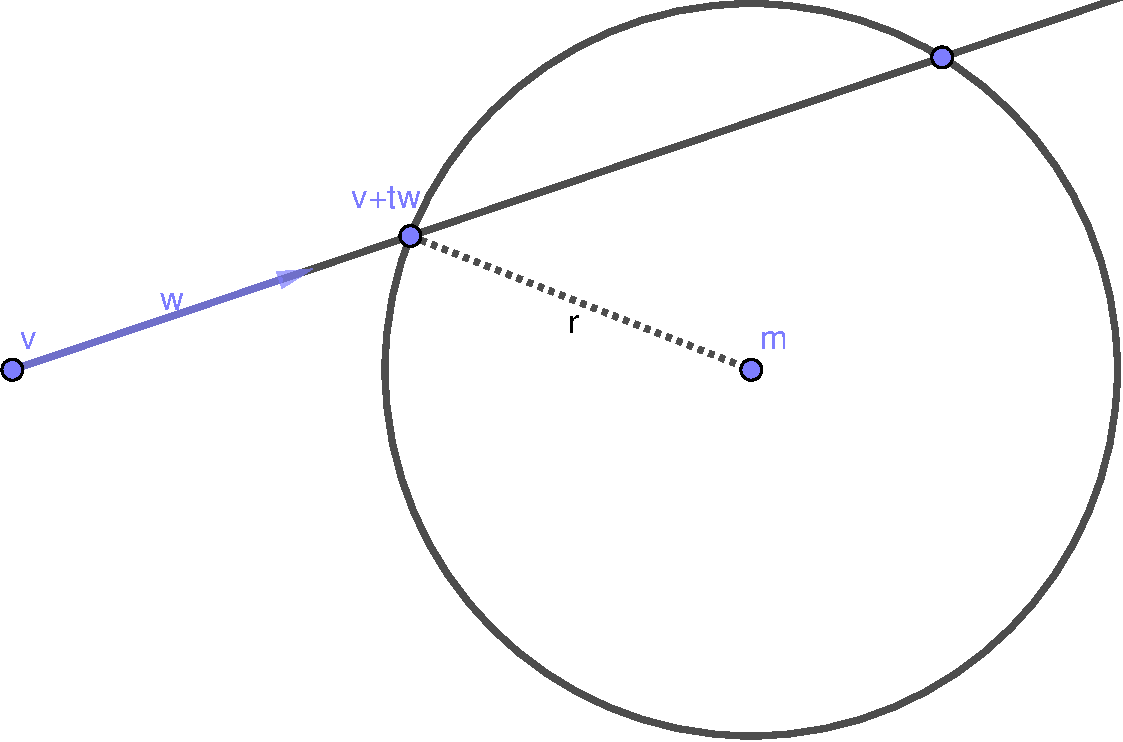
\includegraphics[width=0.5\textwidth]{images/sphere_intersect.pdf}
	\caption{Schnittpunkt von Strahl und Kugel.}
	\label{fig:sphere_intersect}
\end{figure}
\begin{aufgabe}\label{aufg:intersect_theory}
	Gegeben sei eine Kugel mit Mittelpunkt $\vec{m}$ und Radius $r>0$, sowie ein Strahl mit Ursprung $\vec{v}$ und Richtung $\vec{w}$.
	Der Strahl besteht also aus der Menge aller Punkte der Form $\vec{v}+t\vec{w}$ für ein $t>0$.
	Sie dürfen dabei annehmen, dass $\vec{w}$ nicht der Nullvektor ist.
	Wie kann man entscheiden, ob der Strahl die Kugel schneidet?
	Wie erhalten Sie in diesem Fall den Parameter $t>0$, so dass $\vec{v}+t\vec{w}$ gerade dem näherem der beiden Schnittpunkte entspricht?
\end{aufgabe}
\begin{losung*}
	Ein beliebiger Punkt auf dem Strahl ist von der Form $\vec{v}+s\vec{w}$ für ein $s>0$.
	So ein Punkt liegt auf der Kugeloberfläche genau dann wenn
	\begin{equation*}
		\lVert\vec{v}+s\vec{w}-\vec{m}\rVert^2=r^2,
	\end{equation*}
	also wenn er den Abstand $r$ zum Mittelpunkt hat.
	Dies ist eine quadratische Gleichung in $s$, das heisst sie ist von der Form
	\begin{equation*}
		as^2+bs+c=0
	\end{equation*}
	für reelle Zahlen $a,b$ und $c$.
	Durch einen Koeffizientenvergleich erhält man
	\begin{equation*}
		a=\rVert\vec{w}\rVert^2,\quad
		b=2\vec{w}\cdot(\vec{v}-\vec{m}),\quad
		c=\lVert\vec{v}-\vec{m}\rVert^2-r^2.
	\end{equation*}
	Falls $b^2-4ac>0$, so existieren genau zwei Schnittpunkte $v+t_1w$ und $v+t_2w$, wobei
	\begin{equation*}
		t_1=\frac{-b-\sqrt{b^2-4ac}}{2a}
		\quad\text{und}\quad
		t_2=\frac{-b+\sqrt{b^2-4ac}}{2a}.
	\end{equation*}
	Wir sind aber nur an positiven Lösungen interessiert, denn wir beschreiben einen Strahl und keine Gerade.
	Sind $t_1$ und $t_2$ beide negativ, so schneidet der Strahl die Kugel nicht.
	Andernfalls ist die kleinste positive Lösung der quadratischen Gleichung unsere Wahl für $t$.
	Der nächstgelegene Schnittpunkt ist entsprechend $\vec{v}+t\vec{w}$.
\end{losung*}
\begin{aufgabe}\label{aufg:intersect_implementation}
	Öffnen Sie nun das File \texttt{myobject/sphere.py} und implementieren Sie die Funktion \texttt{intersect(self, ray)} gemäss Ihren Überlegungen aus Aufgabe~\ref{aufg:intersect_theory}.
	Lassen Sie anschliessend das Skript \texttt{examples/example1.py} nochmals laufen.
	Nun sollten Sie die Kugel sehen.
\end{aufgabe}
\begin{losung*}
	Die Lösung könnte zum Beipiel so aussehen:
	\lstinputlisting[style=python,linerange=intersect\-begin-intersect\-end]{../object/sphere.py}
	Zusätzlich zu unserer Lösung von Aufgabe~\ref{aufg:intersect_theory} haben wir hier noch überprüft, ob der Strahl am Schnittpunkt in die Kugel eintritt (und nicht etwa austritt).
	Nur diese Lösung lassen wir zu.
	Wir werden später sehen, warum das nützlich ist.
	Das so generierte Bild ist in Abbildung~\ref{fig:solution_sphere} gezeigt.
	\begin{figure}[ht]
		\centering
		\includegraphics[width=0.5\textwidth]{images/example1.png}
		\caption{Lösung der Aufgabe~\ref{aufg:intersect_implementation}.}
		\label{fig:solution_sphere}
	\end{figure}
\end{losung*}
Unsere Kugel sieht momentan eher wie eine Kreisscheibe aus, weil wir der Kugel an jedem Punkt den selben Farbwert geben.
Das wollen wir nun ändern indem wir eine diffuse Lichtreflexion simulieren.
Das Python-File \texttt{examples/example2.py} platziert zu diesem Zweck eine Punktförmige Lichtquelle an den Koordinaten $(0,0,10)$.
Diese wollen wir nun in die Berechnung der Farbwerte miteinbeziehen:
Die Punkte auf der Kugeloberfläche, welche der Lichtquelle zugewandt sind, sollen heller sein.
Die wichtigsten Begriffe sind das \textit{Skalarprodukt} und der \textit{Normalenvektor} auf die Kugeloberfläche.
Man betrachte dazu Abbildung~\ref{fig:sphere_diffuse}.
Diese zeigt eine punktförmige Lichtquelle am Ort $\vec{l}$.
Wir wollen den Farbwert am Punkt $\vec{p}$ auf der Kugel berechnen.
Der Vektor $\vec{n}$ an diesem Punkt soll rechtwinklig zur Kugeloberfläche sein, nach aussen Zeigen und Länge $1$ haben.
Wir nennen $\vec{n}$ den Normalenvektor auf die Kugel im Punkt $\vec{p}$.
\begin{figure}[ht]
	\centering
	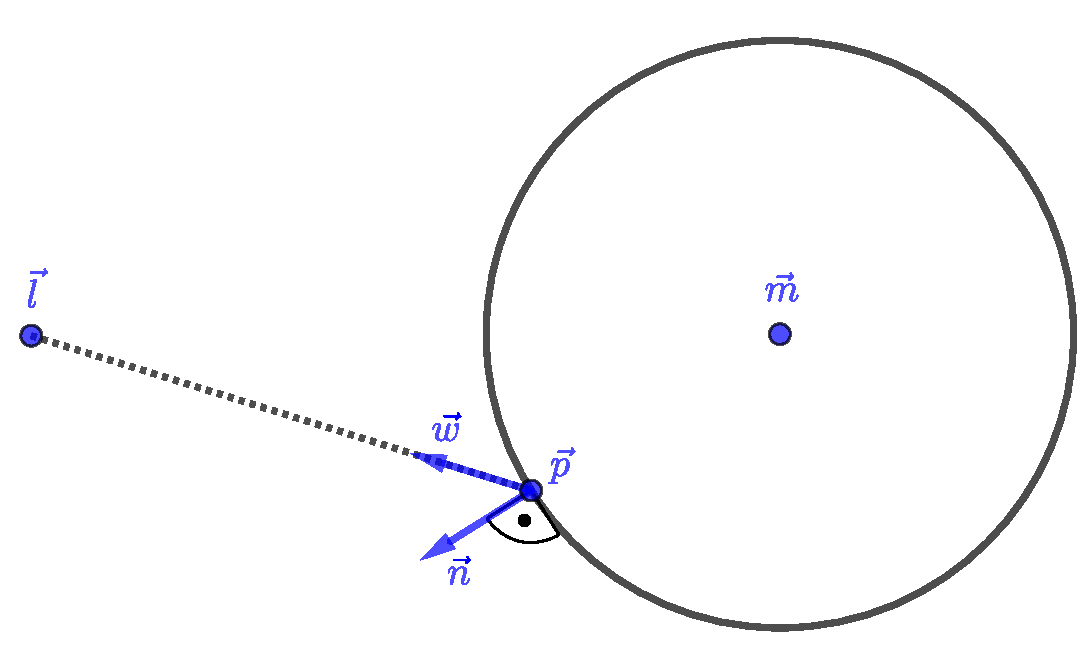
\includegraphics[width=0.5\textwidth]{images/sphere_diffuse.pdf}
	\caption{Die Kugel wird von einer Punktförmigen Lichtquelle in $\vec{v}$ beleuchtet.}
\label{fig:sphere_diffuse}
\end{figure}
Wir ordnen dem Punkt $\vec{p}$ eine Zahl $c\in\left[0,1\right]$ zu, welche die \glqq Helligkeit\grqq an diesem Punkt beschreibt.
Dabei bedeutet $c=1$ maximale Helligkeit und $c=0$ minimale Helligkeit, also schwarz:
\begin{equation}\label{eq:diffuse_coefficient}
	c=\max\left(\vec{n}\cdot\vec{w}, 0\right),\quad
	\vec{w}=\frac{\vec{l}-\vec{p}}{\lVert\vec{l}-\vec{p}\rVert}.
\end{equation}
\begin{aufgabe}\label{aufg:diffuse_coefficient}
	Überlegen Sie sich qualitativ, welche Punkte $\vec{p}$ auf der Kugeloberfläche welchen Wert für $c$ zugeordnet bekommen.
	Welche Punkte auf der Kugeloberfläche werden als \glqq hell\grqq{} und welche als \glqq dunkel\grqq{} erscheinen?
\end{aufgabe}
\begin{losung*}
	Da sowohl $\vec{n}$ als auch $\vec{w}$ Länge $1$ haben, gilt
	\begin{equation*}
		\cos\left(\alpha\right)=\vec{n}\cdot\vec{w},
	\end{equation*}
	wobei $\alpha$ der Zwischenwinkel von $\vec{n}$ und $\vec{w}$ ist.
	Da der Kosinus nur Werte in $\left[-1,1\right]$ annimmt, gilt wie verlangt $c\in\left[0,1\right]$.
	Die Helligkeit hängt also vom Einfallswinkel des Lichtes ab:
	Scheint das Licht rechtwinklig auf die Kugeloberfläche im Punkt $\vec{p}$, so haben wir $\alpha=0$ und damit $c=1$, also maximale Helligkeit.
	Je flacher der Einfallwinkel des Lichtes, desto kleiner wird $c$, bis schliesslich alle  Punkte auf der der Lichtquelle abgewandten Seite die Helligkeit $c=0$ haben.
\end{losung*}
\begin{aufgabe}\label{aufg:diffuse_implementation}
	Öffnen Sie nun das File \texttt{myobject/sphere.py} und implementieren Sie die Funktion \texttt{get\_normal(self, p)}, nach aussen zeigenden Normalenvektor $\vec{n}$ der Lange $1$ am Punkt $\vec{p}$ zurück gibt.
	Lassen Sie anschliessend das Skript \texttt{examples/example2.py} laufen.
\end{aufgabe}
\begin{losung*}
	Die Lösung könnte zum Beipiel so aussehen:
	\lstinputlisting[style=python,linerange=get\_normal\-begin-get\_normal\-end]{../object/sphere.py}
	Das generierte Bild in Abbildung~\ref{fig:solution_diffuse} sieht schon viel interessanter aus.
	Die Lichtquelle befindet sich über der Kugel und beleuchtet nur deren obere Hälfte.
	\begin{figure}[ht]
		\centering
		\includegraphics[width=0.5\textwidth]{images/example2.png}
		\caption{Lösung der Aufgabe~\ref{aufg:diffuse_implementation}.}
		\label{fig:solution_diffuse}
	\end{figure}
\end{losung*}
\end{document}
